\section{Aplicación Móvil (Cliente)}

Una vez que la aplicación es instalada en el dispositivo móvil, es posible comenzar a consumir los servicios ofrecidos por el servidor y hacer uso de las funcionalidades que se tienen disponibles en base a los requerimientos planteados en este documento.
A continuación se muestra la estructura de la aplicación móvil y se detallan las funcionalidades que el usuario tiene a su disposición.

\subsection{Navegación}
La aplicación está compuesta por nueve vistas diferentes, las cuales a su vez, ofrecen diferentes opciones de navegación y configuración que se describirán a detalle. 
Las vistas principales son:
\begin{itemize}
    \item Configuración Personal
    \item Hoteles
    \item Vuelos
    \item Info AICM
    \item Lista de equipaje 
    \item Itinerario de viaje 
    \item Ruta al AICM
    \item Ubícate 
    \item Info vuelo  
    	\end{itemize}

Dichas vistas podrán ser accedidas mediante un menú que se muestra en la vista principal.
\begin{figure}[h]
	\centering
		
\includegraphics[width=0.5\textwidth]{Figuras/main.png}
		\rule{30em}{0.5pt}
	\caption[Vista principal de TASMC]{Vista principal de TASMC}
	\label{fig:vistaprincipalTASMC}
\end{figure}

\begin{figure}[h]
	\centering
		\includegraphics[width=0.5\textwidth]{Figuras/menu.png}
		\rule{30em}{0.5pt}
	\caption[Menú de TASMC]{Menú de TASMC}
	\label{fig:menuTASMC}
\end{figure}
\clearpage

\subsection{Módulo Configuración de la aplicación}
Al iniciar la aplicación por primera vez se muestra una vista en la cual el usuario podrá configurar gustos y preferencias según clase en la que prefiere viajar y categoría de hoteles en los que prefiere hospedarse, esto para facilitar la búsqueda de hoteles y vuelos que este desee, 
además de proporcionar su correo electrónico para posibles sugerencias que el sistema le pueda hacer llegar.
En caso de no realizar su configuración podrá solicitar hacerla más tarde dentro de la vista principal de la aplicación.
\begin{figure}[h]
	\centering
		\includegraphics[width=0.5\textwidth]{Figuras/configuracion.png}
		\rule{30em}{0.5pt}
	\caption[Configuración inicial de TASMC]{Configuración inicial de TASMC}
	\label{fig:configuracionTASMC}
\end{figure}
\clearpage

\subsection{Módulo Hoteles}
Al ingresar al módulo de hoteles se mostrara una vista que contiene un formulario el cual servirá para realizar una búsqueda de hoteles, según los parámetros ingresados como son:

\begin{itemize}
\item Nombre de la ciudad o lugar destino.
\item Número de huéspedes.
\item Número de estrellas del hotel.
\end{itemize}

\begin{figure}[h]
	\centering
		\includegraphics[width=0.5\textwidth]{Figuras/hoteles.jpg}
		\rule{30em}{0.5pt}
	\caption[Buscar Hoteles Disponibles]{Buscar Hoteles Disponibles}
	\label{fig:buscarHoteles}
\end{figure}
\clearpage

\subsubsection{Módulo Hoteles Disponibles}
Al realizar la búsqueda de hotel en la vista de Hoteles se mostrará la información 
referente dependiendo de las características que se hayan ingresado y la disponibilidad que exista, como es:
\begin{itemize}
\item Nombre del hotel.
\item Teléfono.
\item Número de estrellas representado por medio de una imagen.
\end{itemize}
\begin{figure}[h]
	\centering
		\includegraphics[width=0.5\textwidth]{Figuras/hdisponible.png}
		\rule{30em}{0.5pt}
	\caption[Hoteles Disponibles]{Hoteles Disponibles}
	\label{fig:hotelesDisponibles}
\end{figure}

\clearpage

\subsubsection{Módulo Detalle Hotel}
Finalmente se podrá obtener la información completa del hotel seleccionado en la lista de hoteles disponibles. Además se mostrará un 
listado de las distintas habitaciones que ofrece el hotel así como teléfono y página web.

\begin{figure}[h]
	\centering
		\includegraphics[width=0.5\textwidth]{Figuras/detalle.png}
		\rule{30em}{0.5pt}
	\caption[Hoteles Disponibles]{Hoteles Disponibles}
	\label{fig:hotelesDisponibles}
\end{figure}

\clearpage

\subsection{Módulo Vuelos}
Este módulo de vuelos mostrará una vista que contiene un formulario el cual servirá para realizar una búsqueda de vuelos, según los parámetros ingresados como son:

\begin{itemize}
\item Origen.
\item Destino.
\item Fecha de Ida.
\item Clase de vuelo.
\end{itemize}

\begin{figure}[h]
	\centering
		\includegraphics[width=0.5\textwidth]{Figuras/buscav.png}
		\rule{30em}{0.5pt}
	\caption[Buscar Vuelos]{Buscar Vuelos}
	\label{fig:vuelos}
\end{figure}
\clearpage

\subsubsection{Módulo Vuelos Disponibles}
Al realizar la búsqueda de vuelo en la vista de Vuelos se mostrará la información referente dependiendo de las características que se hayan ingresado y la disponibilidad que exista, 
como es:
\begin{itemize}
\item Número de vuelo.
\item Hora de salida y llegada.
\item Origen y destino.
\item Aerolínea.
\end{itemize}

\begin{figure}[h]
	\centering
		\includegraphics[width=0.5\textwidth]{Figuras/vdisponibles.png}
		\rule{30em}{0.5pt}
	\caption[Vuelos Disponibles]{Vuelos Disponibles}
	\label{fig:vuelosDisponibles}
\end{figure}
\clearpage

\subsection{Módulo Información del AICM}
A través de esta vista, el sistema muestra la información referente al AICM tales como sitio web, teléfono, ubicación, mapa y servicios.

\begin{figure}[h]
	\centering
		\includegraphics[width=0.5\textwidth]{Figuras/infoaicm.png}
		\rule{30em}{0.5pt}
	\caption[Información del AICM]{Información del AICM}
	\label{fig:infoAICM}
\end{figure}
\clearpage

\subsubsection{Módulo Mapa del AICM}
Al seleccionar el mapa en el módulo de Información del AICM se mostrar una vista la cual se encuentra divida en dos mapas como es la Planta baja y Planta alta del AICM T1.

\begin{figure}[h]
	\centering
		\includegraphics[width=0.5\textwidth]{Figuras/mapapa.png}
		\rule{30em}{0.5pt}
	\caption[Mapa Planta Alta Terminal 1]{Mapa Planta Alta Terminal 1}
	\label{fig:mapaPA}
\end{figure}

\begin{figure}[h]
	\centering
		\includegraphics[width=0.5\textwidth]{Figuras/mapapb.png}
		\rule{30em}{0.5pt}
	\caption[Mapa Planta Baja Terminal 1]{Mapa Planta Baja Terminal 1}
	\label{fig:mapaPB}
\end{figure}
\clearpage

\subsubsection{Módulo Servicios del AICM}
Al seleccionar los servicios en el módulo de Información del AICM se mostrar una lista de los servicios que ofrece el AICM T1.

\begin{figure}[h]
	\centering
		\includegraphics[width=0.5\textwidth]{Figuras/servicios.png}
		\rule{30em}{0.5pt}
	\caption[Servicios Terminal 1]{Servicios Terminal 1}
	\label{fig:servicios}
\end{figure}
\clearpage

\subsection{Módulo Lista de Equipaje}
Este apartado nos muestra una lista con sugerencias de equipajes con un propósito específico así como la opción de generar nuevas listas propias del viajero. 
Dichas sugerencias de equipaje son cargadas directamente de la aplicación web de administración.

\begin{figure}[h]
	\centering
		\includegraphics[width=0.5\textwidth]{Figuras/equipaje.png}
		\rule{30em}{0.5pt}
	\caption[Listas de Equipaje]{Listas de Equipaje}
	\label{fig:equipaje}
\end{figure}
\clearpage

\subsubsection{Módulo Nuevo Equipaje}
Esta vista se muestra cuando se selecciona crear un nuevo equipaje en el modulo de Lista de Equipaje, 
aquí se solicita un nombre y la selección de diversos objetos que el usuario requiera para su viaje.

\begin{figure}[h]
	\centering
		\includegraphics[width=0.5\textwidth]{Figuras/nuevoequipaje.jpg}
		\rule{30em}{0.5pt}
	\caption[Nuevo Equipaje]{Nuevo Equipaje}
	\label{fig:nuevoEquipaje}
\end{figure}
\clearpage

\subsection{Módulo Itinerario de viaje}
Esta vista muestra una lista de itinerarios de viaje que el usuario haya creado, 
mostrando el destino de viaje así como las actividades a realizar en dicho lugar.

\begin{figure}[h]
	\centering
		\includegraphics[width=0.5\textwidth]{Figuras/itinerario.jpg}
		\rule{30em}{0.5pt}
	\caption[Itinerario de viaje]{Itinerario de Viaje}
	\label{fig:itinerario}
\end{figure}
\clearpage

\subsubsection{Módulo Nuevo Itinerario de viaje}
Una vez que se haya solicitado crear un nuevo itinerario de viaje se mostrara una vista donde se podrán ingresar un destino así como las actividades que desee realizar en su viaje.

\begin{figure}[h]
	\centering
		\includegraphics[width=0.5\textwidth]{Figuras/nuevoiti.png}
		\rule{30em}{0.5pt}
	\caption[Nuevo Itinerario de viaje]{Nuevo Itinerario de Viaje}
	\label{fig:nuevoItinerario}
\end{figure}
\clearpage

\subsection{Módulo Ruta al AICM}
Es la vista que muestra un mapa en la cual se encuentran marcados 3 ubicaciones, como es la ubicación principal del AICM y 
las dos terminales con las que cuenta (T1 y T2) esto con el propósito de ofrecerle al usuario la generación de una ruta desde 
su origen el cual puede ser accedido mediante un botón y en el cual resaltara mediante un marcador táctil dicho origen, 
un botón que llevara a la localización principal del AICM y donde de igual manera el usuario seleccionara mediante otro marcador
la terminal requerida, finalmente se podrá visualizar la ruta hacia el AICM.

\begin{figure}[h]
	\centering
		\includegraphics[width=0.5\textwidth]{Figuras/locaicm.png}
		\rule{30em}{0.5pt}
	\caption[Localización AICM]{Localización AICM}
	\label{fig:localizacionAICM}
\end{figure}

\begin{figure}[h]
	\centering
		\includegraphics[width=0.5\textwidth]{Figuras/loct1.png}
		\rule{30em}{0.5pt}
	\caption[Localización Terminal 1]{Localización Terminal 1}
	\label{fig:localizacionT1}
\end{figure}

\begin{figure}[h]
	\centering
		\includegraphics[width=0.5\textwidth]{Figuras/loct2.png}
		\rule{30em}{0.5pt}
	\caption[Localización Terminal 2]{Localización Terminal 2}
	\label{fig:localizacionT2}
\end{figure}

\begin{figure}[h]
	\centering
		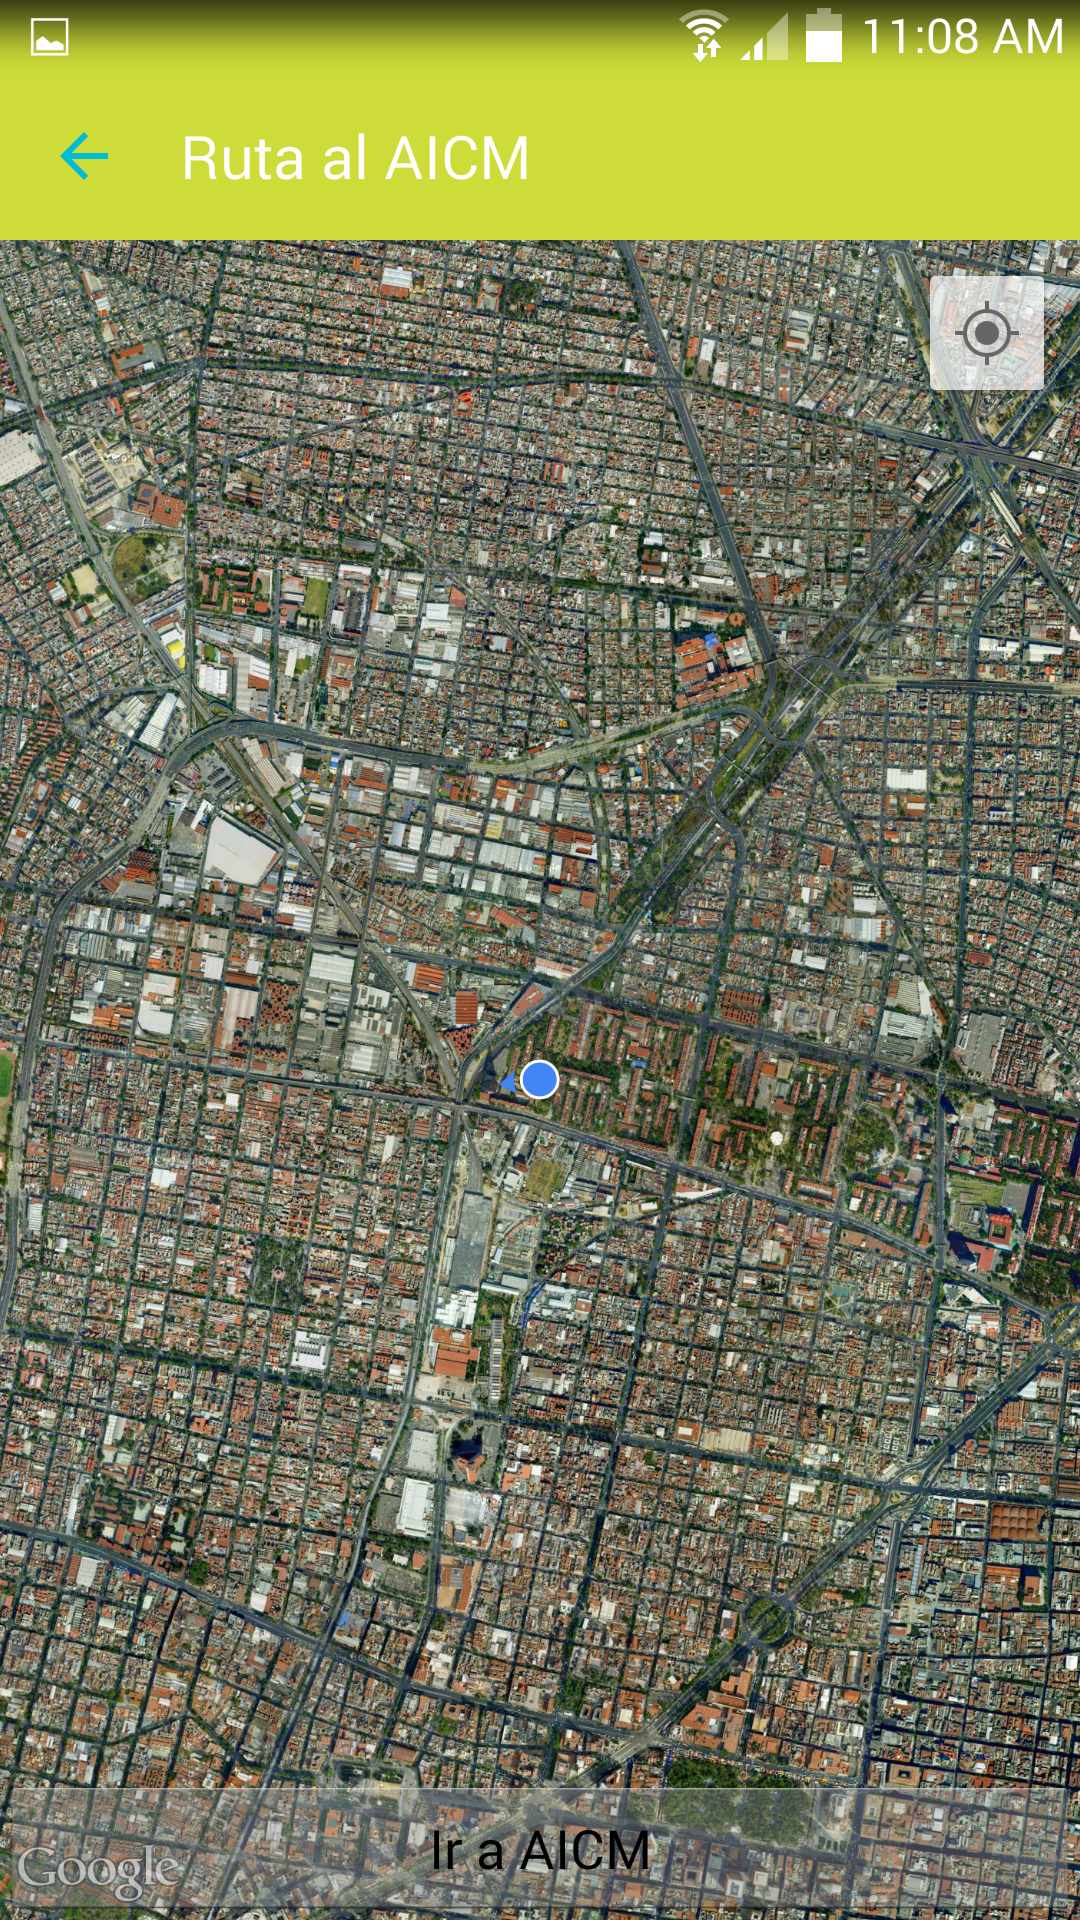
\includegraphics[width=0.5\textwidth]{Figuras/locmia.png}
		\rule{30em}{0.5pt}
	\caption[Ubicación Actual]{Ubicación Actual}
	\label{fig:miUbicacion}
\end{figure}

\begin{figure}[h]
	\centering
		\includegraphics[width=0.5\textwidth]{Figuras/ruta.png}
		\rule{30em}{0.5pt}
	\caption[Ruta al AICM]{Ruta al AICM}
	\label{fig:rutaAICM}
\end{figure}
\clearpage

\subsection{Módulo Localización dentro del AICM}
Dicho apartado contendrá el mapa del interior del AICM como es planta alta y baja de la edificación esto con el propósito de brindar un servicio de localización en interiores, 
el cual le permitirá al usuario localizar su sala de abordaje de una manera más rápida.

\begin{figure}[h]
	\centering
		\includegraphics[width=0.5\textwidth]{Figuras/ubikpa.jpg}
		\rule{30em}{0.5pt}
	\caption[Localización en Planta Alta Terminal 1]{Localización en Planta Alta Terminal 1}
	\label{fig:indoorPA}
\end{figure}

\begin{figure}[h]
	\centering
		\includegraphics[width=0.5\textwidth]{Figuras/ubikpb.jpg}
		\rule{30em}{0.5pt}
	\caption[Localización en Planta Baja Terminal 1]{Localización en Planta Baja Terminal 1}
	\label{fig:indoorPB}
\end{figure}
\clearpage

\subsection{Módulo Información de vuelo}
Esta vista permitirá al usuario consultar la información de salidas y llegadas tanto nacionales como internacionales, 
además de buscar mediante su número de vuelo información referente a su vuelo.

\begin{figure}[h]
	\centering
		\includegraphics[width=0.5\textwidth]{Figuras/llegadas.png}
		\rule{30em}{0.5pt}
	\caption[Información de Llegadas Nacionales e Internacionales]{Información de Llegadas Nacionales e Internacionales}
	\label{fig:infoLlegadas}
\end{figure}

\begin{figure}[h]
	\centering
		\includegraphics[width=0.5\textwidth]{Figuras/salidas.png}
		\rule{30em}{0.5pt}
	\caption[Información de Salidas Nacionales e Internacionales]{Información de Salidas Nacionales e Internacionales}
	\label{fig:infoSalidas}
\end{figure}
\clearpage

\subsubsection{Módulo Información de mi vuelo}
Esta vista mostrará información referente al número de vuelo que ingresado en el módulo de Información de vuelo.

\begin{figure}[h]
	\centering
		\includegraphics[width=0.5\textwidth]{Figuras/mivuelo.png}
		\rule{30em}{0.5pt}
	\caption[Información de vuelo]{Información de vuelo}
	\label{fig:infoVuelo}
\end{figure}
\clearpage


